\documentclass{beamer}

\mode<presentation>
{
\usetheme{Copenhagen}
%\usetheme{Boadilla}
%\usecolortheme{seahorse}
%\useoutertheme{infolines}
%\useoutertheme[compress]{miniframes}
%\setbeamercovered{transparent}
}

%% \mode<presentation>
%% {
%% \usetheme{progressbar}
%% \setbeamercovered{transparent}
%% }

%\usepackage[english]{babel}
\usepackage[english]{babel}
\usepackage[utf8]{inputenc}
\usepackage[T1]{fontenc}

\usepackage{mathptmx}
\usepackage[scaled=.90]{helvet}
\usepackage[T1]{fontenc}
\usepackage{xspace}
%\usepackage{appendixnumberbeamer}
\usepackage[noend]{algorithmic}
%\usepackage[algo2e,vlined,algochapter,ruled,dotocloa]{algorithm2e}
\usepackage{fancybox}
\usepackage{algorithm}
\usepackage[noend]{algorithmic}
\usepackage{amssymb,amsmath}
% \usepackage{ulem}
\usepackage{makecell}
\usepackage{times}
\usepackage{bbding}

\title[A few topics in Reinforcement Learning]{From Field problems to Machine Learning}
\subtitle{An introduction to the Data Science workflow\\and a motivation to understand Machine Learning}
%\title{The Optimal Swapping Problem during Nuclear Refueling Operations}


\author{E. Rachelson}

\institute{
\includegraphics[width=1.5cm]{img/isae.jpg}}

\date{}


\setbeamerfont{bibliography entry author}{shape=\upshape,series=\bfseries,size=\footnotesize}%
\setbeamerfont{bibliography entry title}{shape=\upshape,size=\scriptsize,series=\mdseries}
\setbeamerfont{bibliography entry journal}{shape=\upshape,size=\scriptsize,series=\mdseries}
\setbeamerfont{bibliography entry note}{shape=\upshape,size=\scriptsize,series=\mdseries}

\setbeamercolor{block}{bg=blue,fg=red}

\beamertemplatenavigationsymbolsempty
\setbeamertemplate{footline}[frame number]

\begin{document}

\begin{frame}{A probabilistic approach to ML}
\begin{block}{}
Bayesian approach: find $y$ that maximizes $\mathbb{P}(Y=y|\textrm{data}, X=x)$
\end{block}
This problem of Bayesian inference is hard to solve without additional hypothesis.
\end{frame}

\begin{frame}{A probabilistic approach to ML}
\only<1>{
\begin{block}{Gaussian Processes}
\begin{itemize}
\item Compute the most probable function that passes through the data points, given a priori information about how related two data points are (through a covariance kernel);
\item Also provide a measure of prediction uncertainty in each point;
\item Are computed offline and require an $N\times N$ matrix inversion for $N$ data points in the training set (computationnally costly);
\item Careful engineering of covariance kernels can help incorporate priori knowledge into Gaussian Processes;
\item Are suitable both for regression and classification.
\end{itemize}
\end{block}
}
\only<2>{Note that Gaussian Processes are widely used in preliminary design phases, especially as surrogate models that replace physics computations.

\begin{center}
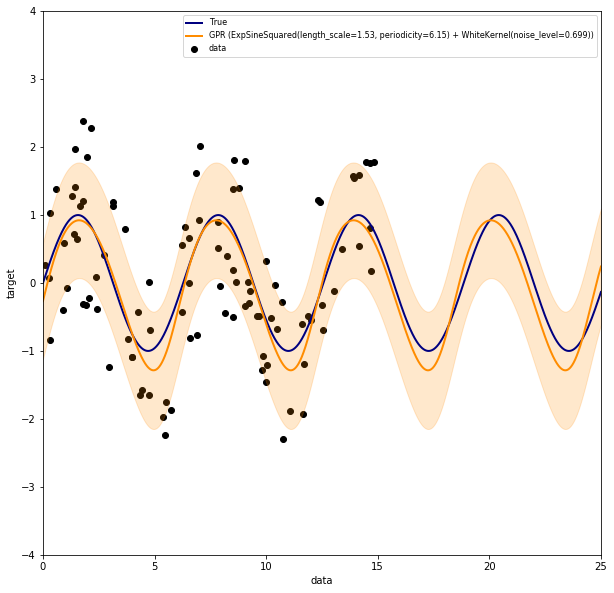
\includegraphics[width=5cm]{img/gaussianprocesses.png}
\end{center}}
\end{frame}

\end{document}
